\documentclass[border=1pt, tikz]{standalone}
\usepackage[rm]{roboto}
%\usepackage[rm,light]{roboto}

\usetikzlibrary{positioning, fit, decorations.text}
%\tikzset{every picture/.style={/utils/exec={\sffamily}}}
\tikzset{every picture/.style={line width=1pt}}

\definecolor{kts-blue}{RGB}{237,241,251}

\begin{document}
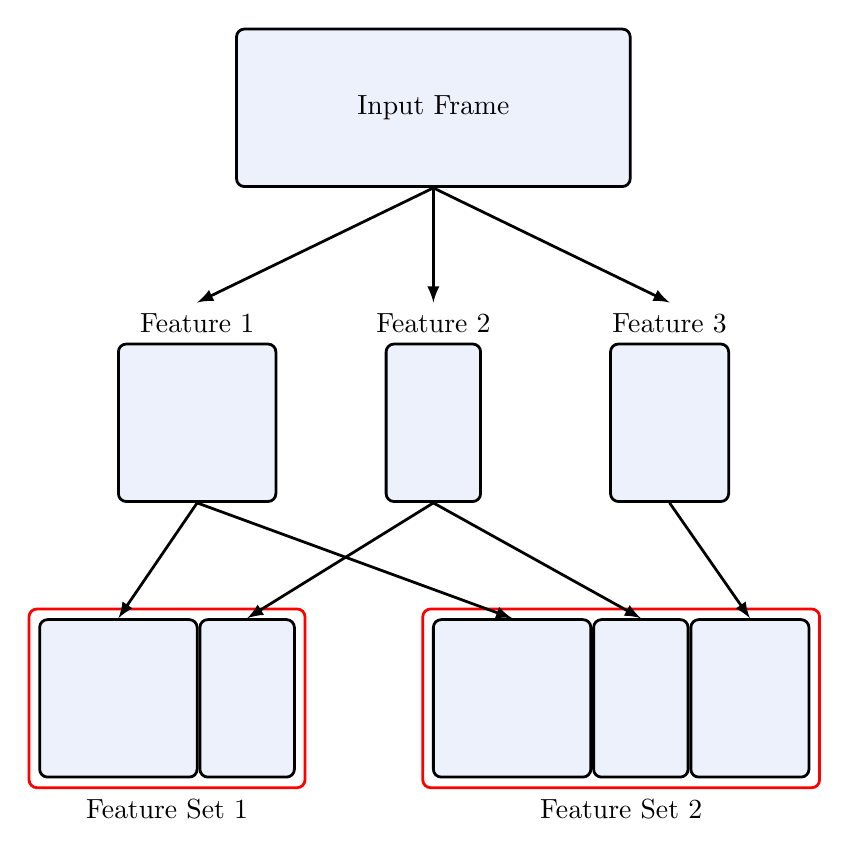
\begin{tikzpicture}
    [rect/.style = {rectangle, draw, align=center, 
            inner xsep=6mm, inner ysep=3mm, fill=kts-blue, rounded corners=0.1cm},
    -latex,     
    fs/.style = {rectangle, draw, align=center, 
            rounded corners=0.1cm},
    -latex,  
    ]
    
	\node[rect, minimum height=2cm, minimum width=5cm] (if) at (0, 0) {Input Frame};
	\node[rect, minimum height=2cm, minimum width=2cm] (f1) at (-3, -4) {};
	\node[rect, minimum height=2cm, minimum width=1cm] (f2) at (0, -4) {};
	\node[rect, minimum height=2cm, minimum width=1.5cm] (f3) at (3, -4) {};
	
	\node[above=0.0cm of f1] (f1-text) {Feature 1};
	\node[above=0.0cm of f2] (f2-text) {Feature 2};
	\node[above=0.0cm of f3] (f3-text) {Feature 3};
	
	\node[rect, minimum height=2cm, minimum width=2cm] (fs1-1) at (-4, -7.5) {};
	\node[rect, minimum height=2cm, minimum width=1cm, right=0.0cm of fs1-1] (fs1-2) {};
	
	\node[rect, minimum height=2cm, minimum width=2cm] (fs2-1) at (1, -7.5) {};
	\node[rect, minimum height=2cm, minimum width=1cm, right=0.0cm of fs2-1] (fs2-2) {};
	\node[rect, minimum height=2cm, minimum width=1.5cm, right=0.0cm of fs2-2] (fs2-3)  {};
	
	\node[fs, draw=red, fit=(fs1-1) (fs1-2)] (fs1) {};
	\node[below=0.0cm of fs1] (fs1-text) {Feature Set 1};
	
	\node[fs, draw=red, fit=(fs2-1) (fs2-3)] (fs2) {};
	\node[below=0.0cm of fs2] (fs2-text) {Feature Set 2};
	
    \draw (if.south) -- (f1-text.north);
    \draw (if.south) -- (f2-text.north);
    \draw (if.south) -- (f3-text.north);
    \draw (f1.south) to (fs1-1.north); 

    \draw (f2.south) to (fs1-2.north); 
    \draw (f1.south) to (fs2-1.north); 
    \draw (f2.south) to (fs2-2.north); 
    \draw (f3.south) to (fs2-3.north); 
\end{tikzpicture}
\end{document}